\documentclass{standalone}
\usepackage{pgfplots}
\pgfplotsset{
compat=1.18, 
trig format=rad, 
ticklabel style = {font=\tiny},
axis equal image,
}

\begin{document}
  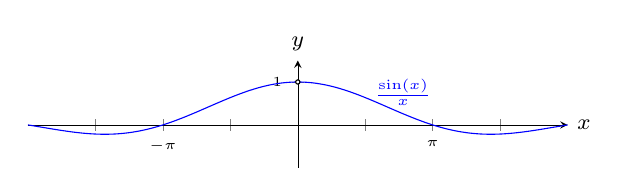
\begin{tikzpicture}
    \begin{axis}[
      axis lines=middle,
      smooth,
      no markers,
      samples=50,
      domain={-2*pi}:{2*pi},
      xlabel={\footnotesize \(x\)},
      xlabel style={at={(ticklabel* cs:1)}, anchor=west},
      ylabel={\footnotesize \(y\)},
      ylabel style={at={(ticklabel* cs:1)}, anchor=south},
      axis line style = {very thin},
      ymin=-1, 
      ymax=1.5, 
      ytick={0,1},
      xtick={-3*pi/2, -pi, -pi/2, 0, pi/2, pi, 3*pi/2},
      % xticklabels={, \(-\pi\), \(-\frac{\pi}{2}\), \(0\), \(\frac{\pi}{2}\), \(\pi\)},
      xticklabels={, \(-\pi\), , \(0\), , \(\pi\)},
      ]
      \addplot[blue]{sin(x)/x};
      \node[right,blue] at (pi/2,0.75) {\tiny \(\frac{\sin(x)}{x}\)};
      \draw[fill=white] (0,1) circle (0.05);
    \end{axis}
  \end{tikzpicture}
\end{document}

